% ADA tagged PDF experiment. Compile with recent LuaLaTeX.
\DocumentMetadata{
  tagging=on,
  tagging-setup={math/setup=mathml-SE},
  pdfstandard=ua-2,
  lang=en-US
}
\documentclass[11pt,letterpaper]{article}
\usepackage[lmargin=2.4in,rmargin=0.5in,tmargin=1.0in,bmargin=1.0in]{geometry}
\usepackage{notes}
\usepackage{unicode-math}
\usepackage{hyperref}
\hypersetup{
  pdflang={en-US},
  pdftitle={Math 316 - 1.1 First-Order Differential Equations},
  pdfauthor={T. Takahashi},
  pdfsubject={Applied Ordinary Differential Equations}
}
\begin{document}


\setlength{\parskip}{6pt}
\begin{center}
\Large\textbf{1.1 – First-Order Differential Equations}\\
\normalsize (Sections 1.1.1, 1.2)
\end{center}

%-------------------------------------------------------------
\section{Differential Equations}

\subsection{Algebraic vs. Differential Equations}
You know how to solve the equation
    \[x^2-x=0\] 
where the unknown variable $x$ is a number $x\in\mathbb{R}$. This is an \textit{algebraic equation}. There are two solutions: $x=0$ and $x=1$. Now consider solving for $x$ in this equation:
  \[ \frac{dx}{dt} - x = 0.\]
You cannot use algebra to solve for $x$ because there is a derivative involved. This is an example of a \textbf{differential equation} (abbreviated as DE). The goal for both equations is the same; solve for $x$. Yet, there is a significant distinction. The answer to an algebraic equation is just a fixed number. However, the answer to a DE is a \textit{function} $x(t)$. A large portion of this course is about learning how to solve DEs.

\subsection{Notations}
We use the Lagrange-style prime notation $(\cdot)'$ for derivatives:
\[
    x' := \frac{dx}{dt}. 
\]
The colon-equal notation $:=$ indicates that a new symbol or variable is being defined, as opposed to stating a new equation. We use additional tick marks for higher order derivatives. For example, the second order derivative is notated as
\[
    x'' := \frac{d^2x}{dt^2}.
\]
The 3rd-order derivative is denoted $x'''$, etc. 

\subsection{Order}
DEs are classified in terms of \textit{order}. The \textbf{order} of a DE refers to the highest order derivative appearing in the equation.
For example, 
\[
    x'''+\sin(x'') - 2x = \sqrt{x} +t 
\]
is a differential equation involving $x'''$ so it is a \textit{3rd order DE}. Increasing the order of a DE typically makes it harder to solve. The first two weeks of the course are about \textit{first-order DEs} 
\[
x' = f(t,x).
\]

\subsection{Verifying Solutions}
The solutions to $x^2-x=0$ are $x=0,1$. To verify these answers, we plug them into the equation and show that the equality holds: 
\begin{align*}
    x^2 - x &=0   &  x^2-x&=0\\
    0-0&=0\; \checkmark   &   1-1&=0 \;\checkmark
\end{align*}
The procedure is the same for DEs. Even if you do not know how to solve a DE, you can still check whether a given solution is valid. Here is an example.

\begin{example}[1]{
Show that the function \[x(t)=e^{t}\] 
is a solution to the DE $x'-x=0$. 
}
We can substitute $x=e^{t}$ into the equation and show that the equation is true:
\begin{align*}
    x' - x &=0\\
    (e^t)'-(e^t)&=0\\
    e^t-e^t&=0\\
    0&=0 \quad \checkmark
\end{align*}
\end{example}

\subsection{General Solution}
We proved that the function $x=e^t$ solves the DE $x'-x=0$, but there's another solution $x=3e^{t}$. You can prove this as well.
% \begin{align*}
%     x' - x &=0\\
%     (3e^{t})'-(3e^{t})&=0\\
%     3e^t-3e^t&=0\\
%     0&=0 \quad \checkmark
% \end{align*}
There is nothing special about the $3$; notice that $x=6e^t$ and $x=7e^t$ are also solutions. In fact, DEs have an \textit{infinite} number of solutions. We can collectively write all solutions as \[x(t) = Ce^{t}\] 
where $C$ represents an arbitrary constant. This function $x(t)=Ce^{t}$ is called the \textbf{general solution} to $x'-x=0$ because it encapsulates the entire set of solutions. General solutions to first-order DEs are always expressed in terms of one arbitrary constant.

%-------------------------------------------------------------
\section{Solving $x'=f(t)$}

In this section, we will start solving some basic DEs. You will have to refresh yourself on integration techniques from Calculus II.

\subsection{The Goal}
We will begin studying the simplest class of DEs.
Our goal is to solve first-order DEs of the form
\[
\frac{dx}{dt} = f(t).
\]
The \textbf{right-hand side} (abbreviated as RHS) of the equation depends only on $t$ and not on $x$. These equations are simple to solve. Consider the two DEs:
\[
x' = \underbrace{3t^2+\cos t+e^t}_{\text{only has }t}, 
\qquad \text{and}\qquad
x' = \underbrace{x^2+\sin t+e^t}_{\text{contains } x\text{ and }t}.
\]
The first is solvable, but the second is impossible.

\subsection{Antiderivative Technique}
To solve $x'=f(t)$, integrate both sides of the equation with respect to $t$:
\begin{align*}
    \frac{dx}{dt} &= f(t)\\
    \int\frac{dx}{dt} \,dt&= \int f(t) \,dt \\
    x(t)&= F(t) +C.
\end{align*}
The function $F(t)$ is the antiderivative of $f(t)$ and $C$ is an arbitrary constant.
Thus, the solution to $x'=f(t)$ is the function
\[
x(t) = \int f(t)\,dt + C.
\]
There isn't a name for this method. I'll refer to it as the \textbf{antiderivative technique}. Let's see an example.

\begin{example}[2]{
Find the general solution to the 
\[
\frac{dx}{dt} = t e^{-2t}.
\]
}
We integrate the RHS using integration by parts 
\begin{align*}    
x(t) &= \int t e^{-2t}\,dt\\ 
    &=\int u\,dv = uv - \int v\,du \qquad (u=t,dv =e^{-2t}dt)\\
    &=-\tfrac12 t e^{-2t} + \int\tfrac12 e^{-2t}\,dt \qquad (du=dt,v =-\tfrac{1}{2}e^{-2t})\\
    &=\boxed{-\tfrac12 t e^{-2t} - \tfrac14 e^{-2t} + C} 
\end{align*}
\end{example}

\subsection{Warning}

Be careful because the antiderivative technique does not work if the RHS contains $x$. For example 
\[
    x' = 3x+\cos(t)
\]
\textit{cannot} be solved with the antiderivative technique. I have seen several  students in the past attempt to solve it anyway. Here's a demonstration of an \emph{incorrect calculation}:
\begin{align*}
    \int x'\,dt &= \int(3x+\cos(t))\,dt\\
    x &= \int 3x\,dt +\int\cos(t)\,dt\\
    x &= \underbrace{ 3xt}_{\text{incorrect}} +\sin t+C
\end{align*}
You can't integrate $\int 3x \,dt$ because $x(t)$ is unknown. Please don't ever do this.
Part of the challenge is knowing the appropriate technique for each situation.

\subsection{Review Integration}
In this class, you will need to review some integration. You are expected to memorize standard integration formulas from Calculus I. For example, 
\[
\int \tfrac{1}{t} \,dt = \ln|t|+C, \quad \text{or} \quad \int \tfrac{1}{t^2+1}dt = \arctan(t)+C.    
\]
You are expected to memorize the following integration techniques from Calculus II:
\begin{itemize}
    \item $u$-substitution
    \item Integration by parts 
    \item Partial fraction decomposition 
\end{itemize}
You will not encounter trig substitution, but you should know how to complete the square. You will have plenty of practice in the first homework.

%-------------------------------------------------------------
\section{Initial Value Problem}

\subsection{Definition}

The set of equations 
\[
\begin{dcases}
    x' = f(t) &\qquad \text{(DE)}\\
    x(t_0) = x_0 &\qquad \text{(IC)}
\end{dcases}
\]
is called the \textbf{initial value problem} (abbreviated as IVP). 
The DE $x'=f(t)$ has an infinite number of solutions. The second equation 
$
x(t_0)=x_0
$
is called the \textbf{initial condition} (abbreviated as IC). The goal of an IVP is to find a single function $x(t)$ that satisfies both the DE and the IC.
Thus, the final answer to this problem will not contain the arbitrary constant $C$.

\subsection{How to solve IVPs}
\begin{enumerate}
    \item First, use the antiderivative technique to find the general solution 
\[
x(t) = F(t) +C.
\]
    \item Next, set up the equation $x(t_0)=x_0$ using your general solution. 
    \item Then solve for $C$. 
    \item Finally, write the solution with the value of $C$.
\end{enumerate}


\begin{example}[3]{    
Find the solution to the initial value problem:
\[
\begin{dcases}
    \frac{dx}{dt}= \frac{2}{t(t+1)}\\
    x(1) = 0
\end{dcases}.
\]
}

Integrating the RHS, requires \textit{partial fraction decomposition}:
\begin{align*}
\text{Let } \frac{2}{t(t+1)} \equiv \frac{A}{t}+ \frac{B}{t+1} &\implies At+A+Bt=2\\
                                                  &\implies \begin{dcases}
                                                      A+B=0\\
                                                      A=2
                                                  \end{dcases}\implies A=2,B=-2.
\end{align*}
Proceeding with the integration:
\begin{align*}    
x(t) = \int \frac{2}{t(t+1)}\,dt &= \int\frac{A}{t}+ \frac{B}{t+1} \;dt\\ 
    &=\int\frac{2}{t}- \frac{2}{t+1}\,dt\\
    &=2\ln t-2\ln|t+1|+C
\end{align*}
Now we apply the initial condition $x(1)=0$ to find the value of $C$. 
\begin{align*}    
x(1) &=2\ln (1)-2\ln2+C\\
 &=0+ -2\ln2 +C \equiv 0 \\
&\implies  C = 2\ln2
\end{align*}
Finally, we write the solution with the value of $C$:
\[
\boxed{
x(t) =2\ln t-2\ln|t+1|-2\ln 2.
}
\]
\end{example}

\subsection{From Solution to IVP}

It is possible to create an IVP for a given solution. A DE is just an equation expressed in terms of $x$, $x'$, and $t$. Here is an example. 

\begin{example}[4]{
Write an IVP for which  
\[ x(t) = te^t\]
is the solution. 
}
    
First, we find the derivative:
\[
    x'(t) = te^t + e^t.
\]
Notice that the function $x$ appears in its own derivative. 
Next, rewrite the derivative in terms of $x$:
\[
x' = te^t + \frac{1}{t} te^t = x + \frac{1}{t}x.
\]
Lastly, we need an IC. We may choose any initial time, such as $t_0=1$. $x(1)=e$. Therefore, an example of an IVP for $x(t)$ is
\[
\boxed{
\begin{dcases}
    x' = x + \frac{1}{t}x\\
    x(1)=e
\end{dcases}.
}
\]
\end{example}

%-------------------------------------------------------------
\section{Fundamental Theorem of Calculus}

The Fundamental Theorem of Calculus (FTC) is one of the most important tools from Calculus I. 
It allows us to build functions directly from integrals and plays an important role in differential equations.

\subsection{Theorem Statement}

\begin{theorem}{Fundamental Theorem of Calculus}
Let $f$ be continuous on $[a,b]$ and define
\[
F(t):=\int_a^t f(s)\,ds.
\]
Then
\[
F'(t)=\frac{d}{dt}\int_a^t f(s)\,ds = f(t).
\]
\end{theorem}

\subsection{Basic Usage}
Here is a basic usage of the FTC:
\[
\frac{d}{dt}\int_2^t \sin(\sqrt{s^2+1})\,ds
=
\sin(\sqrt{t^2+1}).
\]
Notice two important features. The variable inside the integral is $s$, not $t$. After differentiation, we replace $s$ with the upper limit variable $t$.

% \subsection{Interpretation}

% The FTC tells us that integration and differentiation are inverse operations. More importantly, for differential equations, it gives us a systematic way to construct a function whose derivative is prescribed. Suppose we want a function $x(t)$ satisfying
% \[
% x'(t)=f(t).
% \]
% The FTC tells us that
% \[
% x(t)=\int_a^t f(s)\,ds +C
% \]
% is the general solution for any constant $a$. 

\subsection{Combining FTC with Other Rules}

The FTC is often used together with differentiation rules such as the product rule. For example, define
\[
y(t)= t\int_0^t e^s\,ds.
\]
To differentiate $y(t)$, we use the product rule: $\frac{d}{dt}(fg)=f'g+fg'$. Therefore,
\begin{align*}
y'(t)
&=
\frac{d}{dt}\left(t\int_0^t e^s\,ds\right)\\
&=
1\cdot \int_0^t e^s\,ds
+
t\cdot \frac{d}{dt}\int_0^t e^s\,ds\\
&=
\int_0^t e^s\,ds + te^t.
\end{align*}

\subsection{Formal Solutions}

The solution to the IVP
\[
\begin{dcases}
    x' = f(t)\\
    x(t_0)=x_0
\end{dcases}
\]
is the antiderivative of $f(t)$. Using the FTC, we may write the general solution as
\[
x(t) = \int_a^t f(s)\,ds+C. 
\]
The lower limit $a$ can be any number as long as $f(a)$ is well-defined, so we let $a=t_0$. That way, when we apply the initial condition, we get:
\begin{align*}
    x(t_0)&=\int_{t_0}^{t_0} f(s)\,ds +C\equiv x_0\\
          &\implies0 +C = x_0
\end{align*}
The solution to the IVP is
\[
    x(t) =  \int_{t_0}^t f(s)\,ds+x_0. 
\]
It may feel disingenuous to say we have "solved the IVP" because the answer contains an integral. This is called a \textbf{formal solution}, meaning it structurally satisfies the IVP. 

% -------------------------------------

\begin{example}[5]{
Find the formal solution to the initial value problem
\[
\begin{dcases}
    \frac{dx}{dt}= e^{-t^2}\\
    x(2) = 3
\end{dcases}.
\]
}
Note that the function $f(t) = e^{-t^2}$ famously has no closed-form antiderivative. That means it is impossible to write a formula for $\int e^{-t^2}\,dt$. However, we can still write the "formal" antiderivative as 
\[
    x(t) = \int_a^t e^{-s^2}\,ds +C.
\]
Next, we choose the lower limit $a=2$. Applying the IC gives 
\begin{align*}
    x(2) &= \int_2^2 e^{-s^2}\,ds +C\\
    x(2) &= 0 +C  \equiv 3\\
    &\implies C = 3
\end{align*}
The formal solution is 
\[
\boxed{
 x(t)= \int_2^t e^{-s^2}\,ds+3. 
}
\]
\end{example}

% -------------------------------------------

% \subsection{From Function to DE}
% Suppose we define a function to be 
% \[
%     y(t) = t \int_0^t e^s\,ds 
% \]
% which can be thought of a product of two functions $y(t)=f(t)g(t)$. The derivative of $y(t)$ can be found with the product rule 
% \[
% y'(t) = f(t)g'(t) + f'(t)g(t) =  t e^t + \int_0^t e^s\,ds.
% \]
% Notice that we can write the derivative as 
% \[
% y'  =  t e^t + \frac{t}{t}\int_0^t e^s\,ds = te^t + \frac{1}{t}\left( t \int_0^t e^s\,ds\right) = te^t + \frac1t y.
% \]
% What we accomplished is we found a differential equation for the function $y(t):$
% \[
% y' = t e^t+\frac{1}{t} y = f(t,y). 
% \]
% \textit{Takeaway}: We can use the fundamental theorem to find a DE for a function describes in terms of an integral.


% %-------------------------------------------------------------
\section{Physics}

\subsection{Mathematical Model}

Differential equations play an important role in \textit{modeling}. A \textbf{mathematical model} is a differential equation where the unknown function $x(t)$ represents some physical quantity that changes over time. Here are some examples:
\begin{itemize}
    \item $x(t)=$ population of a species after $t$ months,
    \item $x(t)=$ temperature of an object after $t$ minutes,
    \item $x(t)=$ concentration of a chemical after $t$ seconds.
\end{itemize}
By combining $t$, $x$, $x'$, and $x''$ into one equation in a special way, we can enforce the solution to obey physical laws. The easiest example is Newton's 2nd Law.

\subsection{Newton's Law}
Let $x(t)$ be the \textbf{position} of some object in meters after $t$ seconds. Then the derivative $x'(t)$ is the \textbf{velocity} of the object. The second derivative $x''(t)$ is the \textbf{acceleration}. Then \textbf{Newton's Second Law}, in terms of derivatives, is written 
\[
F =mx'',
\]
where $m$ is the mass of the object and $F$ is the force acting on the object. We say that $F=mx''$ is a \textit{model} that describes the motion of an object located at position $x$. Let's see a concrete example.

\subsection{Falling Rock Model}
\textbf{Setup:}
\begin{itemize}
    \item A rock of mass $m$ is released from rest from the top of a 50-meter-tall cliff.
    \item Ignore air resistance. 
    \item Assume gravitational force is acting on the rock 
\[
F=-mg, \quad (g\approx 9.8 \text{ m/s}^2)
\]
\end{itemize}
\textbf{Objective:} find the position of the rock at any given time.\\
\textbf{Modeling:} Let $x(t)$ be the number of meters above ground at time $t$ seconds. Next, we use Newton's Law, and simplify the DE:
\begin{align*}    
F = mx''&=-mg\\ 
\implies x'' &=-g
\end{align*}
% \begin{wrapfigure}{r}{0.5\textwidth}
%     \centering
%     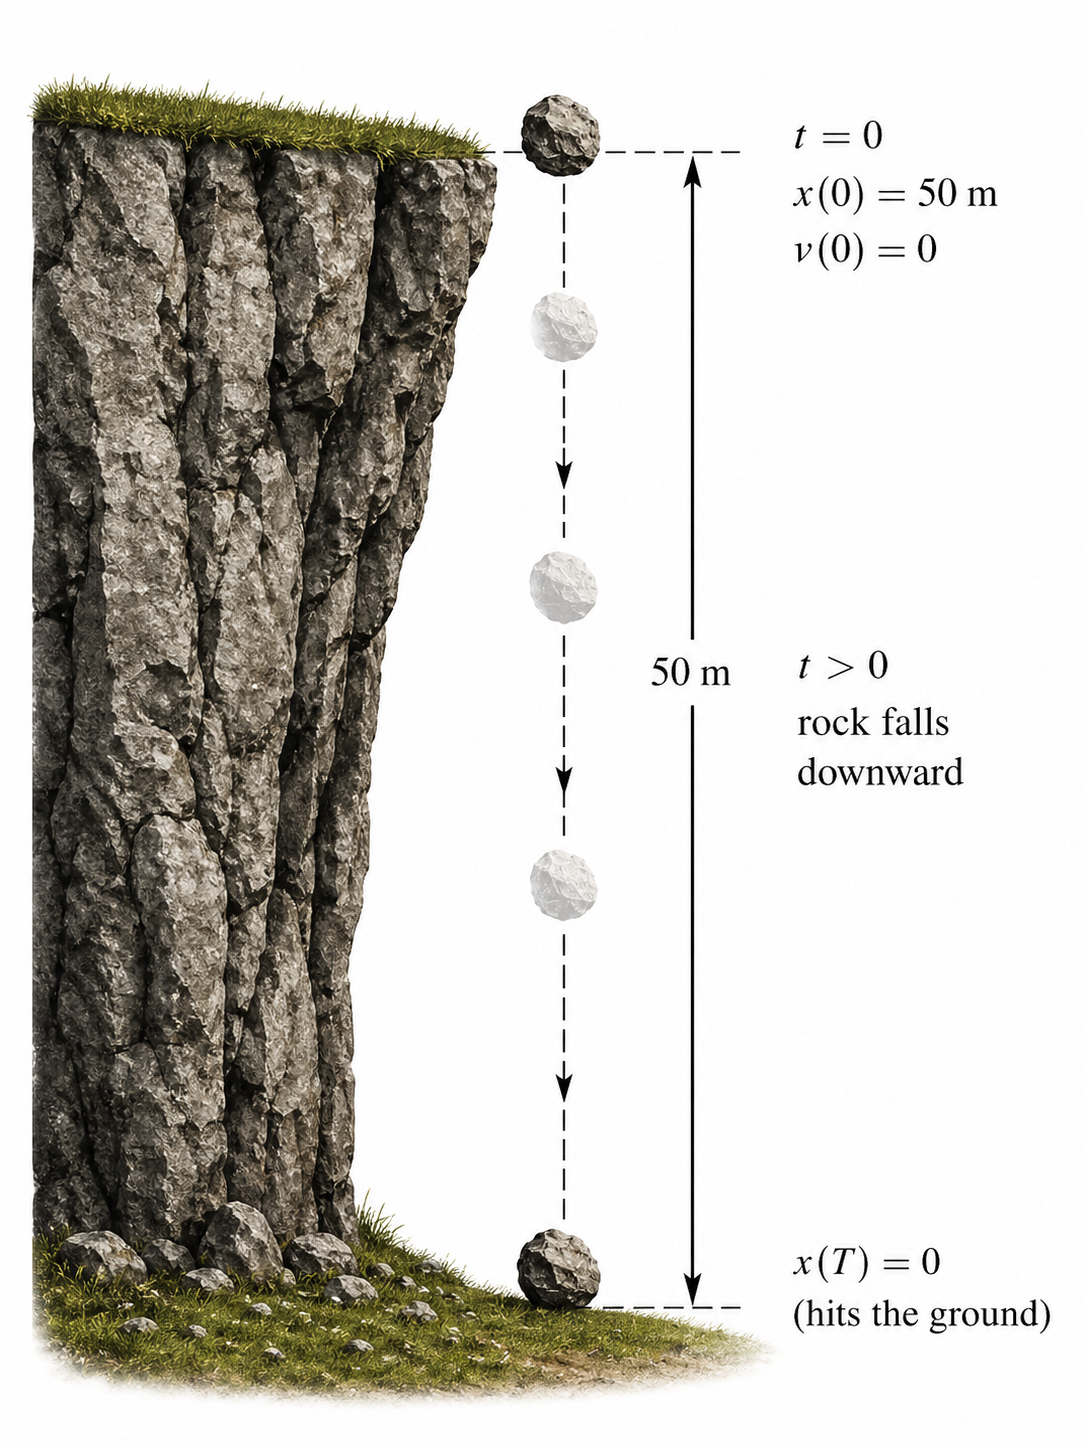
\includegraphics[scale=0.15]{figs/cliff.png}
%     \caption{This is an illustration for the falling rock. The rock picks up speed as it falls due to gravity.}
%     \label{fig:cliff}
% \end{wrapfigure}
Next, we need initial conditions. Since the rock is released from rest from a height of 50 meters, we have
\[
x(0)=50 \text{ m},
\qquad
x'(0)=0.
\]
The mathematical model for the falling rock is therefore
\[
\begin{dcases}
x''(t)=-g,\\
x(0)=50,\\
x'(0)=0.
\end{dcases}
\]
The solution to this IVP is 
\[
x(t) = 50 - \frac{1}{2}gt^2.
\]
This is a powerful function. We know the position of the rock at \textit{any given second}. We can plot the position of the rock as a function of time. We can also determine the time $T$ at which the rock hits the ground. This is a glimpse of what modeling can do.


\subsection{\textit{Applied} ODEs}

Why is this class called \textit{Applied} ODEs? DEs emerged in the 17th century alongside the development of calculus by Newton and Leibniz, largely from problems involving motion and change. Calculus I, II, and III have been a tremendous preparation for math modeling. 

Part of this class is about learning techniques to solve DEs. There is plenty of ``solve this equation using that technique.'' It is very similar to your previous math classes. The other part is about studying models from science and making physical interpretations of their solutions. By the end of the course, you should be able to understand both the mathematics and what it tells us about a real system.


\end{document}
